% #############################################################################
% ################################################## Primary LaTeX Control File
% #############################################################################

\documentclass[11pt, oneside]{mnthesis}

% When creating final version, comment this line out. 
\draft

% =============================================================================
% ============================================================== LaTex Packages
% =============================================================================

% Some of these may not be in use -- but it's safer to leave them than it is to
% remove them and have something break. 
\usepackage{epsfig} % Allows the inclusion of eps files
\usepackage{epic} % Enhanced picture mode
\usepackage{eepic} % Extensions for epic
\usepackage{units} % SI unit typesetting
\usepackage{url} % URL handling
\usepackage{longtable} % Tables that continue onto multiple pages
\usepackage{mathrsfs} % Support for \mathscr script
\usepackage{multirow} % Span rows in tables
\usepackage{amssymb} % AMS math symbols and helpers
\usepackage{graphicx} % Enhanced graphics support
\usepackage{setspace} % Adjust spacing in captions, single by default
\usepackage{xspace} % Automatically adjusting space after macros
\usepackage{amsmath} % \text, and other math formatting options
\usepackage{siunitx} % \num{} formatting and SI unit formatting
\usepackage{booktabs} % Enhanced tables with \toprule, etc.
\usepackage{hyperref} % Add clickable links to other parts of the document
\usepackage[noabbrev,capitalize]{cleveref} % Automatically determine \cref type
\usepackage[hang,flushmargin]{footmisc} % Prevent indent in footnotes. 
\usepackage{lineno} % In draft mode, number lines 
\usepackage{xcolor} % Allows color text for \todo
\usepackage{doi} % Link to doi in the bibliography. Doesn't seem to work. 
\usepackage{parskip} % http://ctan.org/pkg/parskip vskip instead of indent
\usepackage{float} % Allows [H] for telling LaTeX to put an image HERE!
\usepackage[section]{placeins} % Prevetn figures before the start of a section

% =============================================================================
% =============================================================== Configuration
% =============================================================================

% Try to prevent dangling parts of paragraphs over page breaks. 
\widowpenalty10000
\clubpenalty10000

% Configure the siunitx package
\sisetup{
    group-separator = {,}, % Use , to separate groups of digits, like 12,345
    list-final-separator = {, and } % Always use the serial comma in \SIlist
}

% Configure the cleveref package
\newcommand{\creflastconjunction}{, and } % Always use the serial comma

% Bring in the macros defined in my_definitions.tex

% Macros are useful for anything that comes up often. They are defined here,
% and can then be used throughout the document. 

% Bright red reminder. 
\newcommand{\todo}[1]{ \textcolor{red}{TODO --- #1} }

% \ensuremath and \xspace are useful, but sometimes frowned upon. There are 
% some corner cases where they don't behave as expected. 

% Make to-do notes show up in red. 
\newcommand{\dft}[1]{\ensuremath{\overset{\sim}{#1}}\xspace}

% Real and Imaginary prefixes. 
\newcommand{\real}{\ensuremath{\mathbb{R}\mathrm{e}}\xspace}
\newcommand{\imag}{\ensuremath{\mathbb{I}\mathrm{m}}\xspace}

% Names which include special characters. 
\newcommand{\Alfven}{Alfv\'en\xspace}
\newcommand{\Ampere}{Amp\`ere\xspace}
\newcommand{\Schrodinger}{Schr\"odinger\xspace}

% Not sure if it's "Ohm's law" or "Ohm's law"? Use a macro and it's easy to
% change later. 
\newcommand{\ohmlaw}{Ohm's law\xspace}
\newcommand{\amplaw}{\Ampere's law\xspace}
\newcommand{\farlaw}{Faraday's law\xspace}
\newcommand{\maxeqs}{Maxwell's equations\xspace}

% Use underline to indicate vectors and double-underline for tensors. The \vec
% function is already defined -- this overwrites it. 
\renewcommand{\vec}[1]{\ensuremath{\underline{#1}}}
\newcommand{\tensor}[1]{\ensuremath{\underline{\underline{#1}}}}

% Differential operator shortcuts. 
\newcommand{\dd}[1]{\ensuremath{ \frac{\partial}{\partial #1} }\xspace}
\newcommand{\ddt}{\dd{t}\xspace}
\newcommand{\curl}[1]{\ensuremath{ \nabla \times \vec{#1} }\xspace}
\renewcommand{\div}[1]{\ensuremath{ \nabla \cdot \vec{#1} }\xspace}
\newcommand{\grad}[1]{\ensuremath{ \nabla #1 }\xspace}

% Properly-sized matching left and right parentheses. 
\newcommand{\lr}[1]{ \left( #1 \right) }

% Squish "\delta t" together a bit to make it look better. 
\newcommand{\dt}{\ensuremath{\delta \hspace{-0.1em} t}\xspace}

% For the \SI command, make eV look better by shifting it slightly left. 
\DeclareSIUnit\electronvolt{e\hspace{-0.08em}V}

% Plasma frequency, Alfven speed, and other terms that show up a lot in
% dispersion relations. 
\newcommand{\op}{\ensuremath{\omega_P}\xspace}
\newcommand{\va}{\ensuremath{v_A}\xspace}
\newcommand{\ep}{\ensuremath{\epsilon_\bot}\xspace}
\newcommand{\ez}{\ensuremath{\epsilon_0}\xspace}
\newcommand{\mz}{\ensuremath{\mu_0}\xspace}
\newcommand{\oomz}{\ensuremath{ \frac{1}{\mz} }\xspace}
\newcommand{\sz}{\ensuremath{\sigma_0}\xspace}
\newcommand{\sh}{\ensuremath{\sigma_H}\xspace}
\renewcommand{\sp}{\ensuremath{\sigma_P}\xspace}

% Shorthand for a 2x2 matrix. Used as (whitespace/newlines optional):
% \mm{\cos\theta}{\-sin\theta}
%    {\sin\theta}{\cos\theta}
\newcommand{\mm}[4]{ \left[ \begin{array}{cc}
    #1 & #2 \\
    #3 & #4
  \end{array} \right] }

% 3x3 matrix. 
\newcommand{\mmm}[9]{ \left[ \begin{array}{ccc}
    #1 & #2 & #3 \\
    #4 & #5 & #6 \\
    #7 & #8 & #9
  \end{array} \right] }

% 2x1 matrix, or 2-vector. 
\newcommand{\vv}[2]{ \left[ \begin{array}{c}
    #1 \\
    #2
  \end{array} \right] }





% Spacing in LaTeX is weird. This is whatever the style guide asks for. 
\linespread{1.3}

% Drafts have numbered lines. 
\ifdraft
  \linenumbers
\fi

% Set bibliography style -- references are ordered alphabetically, not by the
% order in which they are cited. 
\bibliographystyle{abbrv}

% =============================================================================
% =========================================================== Document Contents
% =============================================================================

\begin{document}

% The abstract, etc, are all handled by title.tex
%%%%%%%%%%%%%%%%%%%%%%%%%%%%%%%%%%%%%%%%%%%%%%%%%%%%%%%%%%%%%%%%%%%%%%%%%%%%%%%%
% title.tex - Set up the beginning of thesis.
%%%%%%%%%%%%%%%%%%%%%%%%%%%%%%%%%%%%%%%%%%%%%%%%%%%%%%%%%%%%%%%%%%%%%%%%%%%%%%%%

% Uncomment to turn on draft mode, which changes the title page to have a draft
% label and date of compilation
%\draft

% Set the type of thesis
\phd % use if for a Ph.D. dissertation
%\ms % use if for a Master of Science thesis

% Set the title and your name. Remember that the guidelines state:
%
% "The title of the thesis must not contain chemical or mathematical formulas,
% symbols, superscripts, subscripts, Greek letters, or other non-standard
% characters; words must be substituted."
\title{\bf Title}
\author{Author Name}
% Advisor name, put co-advisors here as well separated by commas
\director{Advisor Name}

% Specify the month and year; if commented out then these default to the
% current month and year
\submissionmonth{January}
\submissionyear{2106}

% Pages after the title page
\abstract{% #############################################################################
% #################################################################### Abstract
% #############################################################################

\todo{$\cdots$}

}

% Copyright: Uncomment one of the following:
%\copyrightpage       % Full copyright
%\copyrightpageccby   % Full copyright with Creative Commons CC-BY 4.0 license
\copyrightpageccbysa % Full copyright with Creative Commons CC-BY-SA 4.0 license

\acknowledgements{% #############################################################################
% ############################################################ Acknowledgements
% #############################################################################

\todo{$\cdots$}


}
\dedication{% #############################################################################
% ################################################################## Dedication
% #############################################################################

\todo{$\cdots$}



}

% Use a special preface
%\extra{\input{preface}}

% The \beforepreface command actually causes insertion of the title,
% abstract, signature, and copyright pages into the new document.
\beforepreface

% Define the text to go before the table of contents
\figurespage
\tablespage

% The \afterpreface command actually causes insertion of the
% contents, list of figures, etc. into the new document.
\afterpreface
%%%%%%%%%%%%%%%%%%%%%%%%%%%%%%%%%%%%%%%%%%%%%%%%%%%%%%%%%%%%%%%%%%%%%%%%%%%%%%%%


% #############################################################################
% ######################################################## Van Allen Probe Data
% #############################################################################

\chapter{Data}
  \label{ch_data}

Some data is shown in \cref{fig_mode_all_sharp} --- look how great it is! 

Also, check out \cref{tab_iaga}, an example table. These values come from
Jacobs\cite{jacobs_1964}. 

\begin{longtable}{cccccccc}
  \caption[IAGA Magnetic Pulsation Frequency Bands]
    {IAGA Magnetic Pulsation Frequency Bands}
  \label{tab_iaga} \\
  \toprule
  & Pc1 & Pc2 & Pc3 & Pc4 & Pc5 & Pi1 & Pi2 \\
  \midrule
  \endfirsthead
  \bottomrule
  \endlastfoot
  Period (\si{\second}) & 0.2--5    & 5--10    & 10--45  & 45--150 & 150--600 &
    1--40    & 40--150 \\
  Frequency (\si{\mHz}) & 200--5000 & 100--200 & 22--100 & 7--22   & 2--7     &
    25--1000 & 7--25 \\
\end{longtable}

\begin{figure}[!htb]
  \centering
  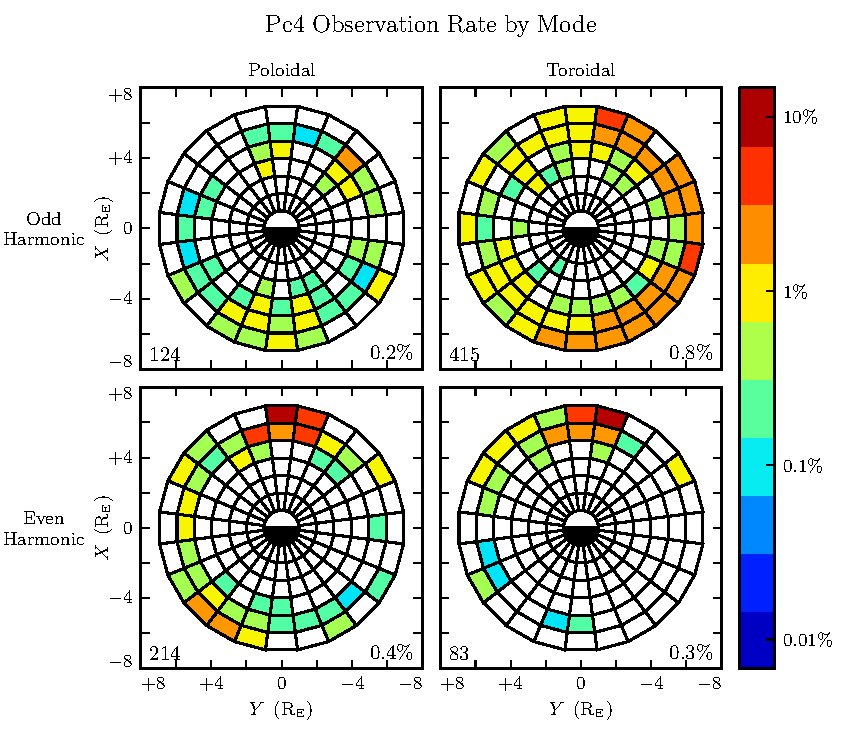
\includegraphics[width=\textwidth]{figures/mode_all_sharp.pdf}
  \caption[Observation Rate of Pc4 Events by Mode]{
    The above figure shows the spatial distribution of Pc4 events observed by
    the Van Allen probes, partitioned by harmonic and polarization. Event
    counts are given in the bottom-left corner. Rates are normalized according
    to the amount of sampling in each bin. Mean rate (assuming a uniform
    spatial sampling) is shown in the bottom-right corner. 
  }
  \label{fig_mode_all_sharp}
\end{figure}


% Assemble the bibliography using dissertation.bib
\bibliography{dissertation}

% Include appendices, if any. 
\appendix
% #############################################################################
% ############################################################## Appendix: Math
% #############################################################################

\chapter{Math}
  \label{app_math}

As you may recall from \cref{ch_data}, there was some data. 

Now let's look at some math. It's based on work by Lysak\cite{lysak_2013}. 

More on that in \cref{sec_maxeqn}

% =============================================================================
% =============================================================================
% =============================================================================

\section{Maxwell's Equations}
  \label{sec_maxeqn}

Start with \amplaw, swapping out the current for $\; \tensor{\sigma} \cdot 
\vec{E} \;$ per Kirchhoff's formulation of \ohmlaw. Finagle a bit to get it
into a form where we can use an integrating factor. 
\begin{align}
  \tensor{\epsilon} \cdot \ddt \vec{E} &= \oomz \curl{B} -
    \tensor{\sigma} \cdot \vec{E}
\end{align}

This can be finagled to:
\begin{align}
  \label{eqn_intfac_0}
  \lr{ \tensor{\Omega} + \tensor{ \mathbb{I} } \ddt } \cdot \vec{E} &=
    \tensor{V}^2 \cdot \vec{F}
\end{align}

Where $\tensor{ \mathbb{I} }$ is the identity tensor, 
${\vec{F} \equiv \curl{B}}$ and in dipole $x$-$y$-$z$ coordinates, 
\begin{align}
  \label{eqn_intfac_1}
  \tensor{V}^2 &\equiv \oomz \tensor{\epsilon}^{-1} = 
    \mmm{\va^2}{0}{0}
        {0}{\va^2}{0}
        {0}{0}{c^2} &
  & \text{and} &
  \tensor{\Omega} &\equiv \tensor{\epsilon}^{-1} \cdot \tensor{\sigma} = 
    \mmm{ \frac{\sp}{\ep} }{ \frac{-\sh}{\ep} }{0}
        { \frac{\sh}{\ep} }{ \frac{\sp}{\ep} }{0}
        {0}{0}{ \frac{\sz}{\ez} } 
\end{align}

Multiplying through by $\exp \lr{ \tensor{\Omega} \, t }$ and applying the
product rule, \cref{eqn_intfac_1} becomes\footnote{Tensor exponentiation is
analogous to scalar exponentiation\cite{hall_2015}:
$\exp\lr{\tensor{T}} \equiv \displaystyle\sum_n \frac{1}{n!} \tensor{T}^n$. }
\begin{align}
  \label{eqn_intfac_2}
  \ddt \Big( \exp \arg{\tensor{\Omega} \, t} \cdot \vec{E} \, \Big) &=
    \exp \lr{\tensor{\Omega} \, t} \cdot \tensor{V}^2 \cdot \vec{F}
\end{align}

\cref{eqn_intfac_2} can then be integrated over a small time step \dt. Note
that in \cref{eqn_intfac_3}, the $\leftarrow$ operator indicates assignment;
values on the left are new, and those on the right are old. 
\begin{align}
  \label{eqn_intfac_3}
  \vec{E} &\leftarrow \exp \arg{ -\tensor{\Omega} \, \dt } \cdot \vec{E} +
    \dt \, \exp \arg{ -\tensor{\Omega} \, \tfrac{\dt}{2} } \cdot
    \tensor{V}^2 \cdot \vec{F}
\end{align}

Now there's something we can plug into the computer! 






\end{document}


